%\documentclass[10pt]{article}

\section{Programa lectura.asm}

El código del programa se encuentra en un único archivo llamado \textbf{lectura.asm}.
Este programa funciona mediante una aplicación de consola usando la api de 32
bits de Windows. Para la lectura del archivo se usan las funciones
CreateFile en modo lectura, GetFileSize y ReadFile el tamaño. GetFileSize
se utiliza para crear un bloque de memoria lo suficientemente grande
para almacenar el archivo en memoria, mas el nuevo registro. Para escribir
el archivo una vez modificado se utilizan lstrlen para poder saber la cantidad
de bytes a escribir y finalmente se usa WriteFile.


El programa se puede dividir en los siguientes pasos:
\begin{itemize}
    \item Apertura y lectura del archivo.
    \item Apertura del archivo en el que se va a escribir.
    \item Conteo de lineas.
    \item Pedir por pantalla los datos que se van a ingresar.
    \item Creacion del nuevo elemento que se anexara al archivo.
    \item Localizacion de la posicion en la que se escribira.
    \item Escritura y cierre del fichero.
\end{itemize}

\subsection*{Apertura y lectura del archivo}

    Para esto se pide por teclado el nombre del fichero a abrir, mediante un
    macro \textbf{Get\_Input} el cual hace uso de las funciones \textbf{StdOut}
    y \textbf{StdIn} para dar como salida un mensaje y leer por teclado.
    Y se utilizan las funciones \textbf{CreateFile, GetFileSize, GlobalAlloc,
    ReadFile} de la misma forma que en la \Cite{pract4} para abrir y almacenar
    la informacion contenida en el archivo y \textbf{CloseHandle} para cerrarla.

\subsection*{Apertura del archivo en el que se va a escribir}

    Una vez tenida la informacion, se abre un nuevo fichero, en este caso en
    modo escritura, para almacenar allí la informacion. Esto se logra con:

    \begin{Verbatim}
       "invoke  CreateFile,ADDR new_file ,GENERIC_WRITE,0,0,\
                CREATE_ALWAYS,FILE_ATTRIBUTE_NORMAL,0
        mov     hFileWrite,eax"
    \end{Verbatim}

    De donde resalta el uso de un nuevo \comillas{handler} y los parametros
    \comillas{ADDR new\_file}, \comillas{GENERIC\_WRITE} y \comillas{CREATE\_ALWAYS}
    las cuales implican el nombre con el que se creara el archivo, el metodo de
    escritura y la opcion de que, aunque el archivo ya exista, siempre se creara
    desde 0.

\subsection*{Conteo de lineas}

    Para el calculo de lineas, se utiliza como contador el registro \textbf{ecx}
    inicializado en 1, la direccion de la informacion en el registro \textbf{esi}
    y se hace un ciclo de chequeo, en el que se recorren todos los caracteres
    del archivo buscando el caracter de salto de linea \textbf{$\backslash$ n} o
    el numero 10 por ascii. Cada vez que hay una coincidencia se incrementa en
    1 el contador, ya que hay una nueva linea, de esta forma cada coincidencia
    implicaria el comienzo de la 2da, 3ra, $\cdots$ , n-esima linea.

    Una vez recorrido todo el archivo, se procede a agregar la linea adicional,
    la nueva a agregar, y por esto se incrementa el contador nuevamente. Se
    guarda el valor obtenido en la pila, mediante un push y se llama al
    procedimiento NumbToStr para guardar el numero convertido en forma de string
    y poder mostrarlo por pantalla cuando se requieran los valores a ingresar.

    Este procedimiento se basa en la construccion del string mediante la obtencion
    individual de cada digito. Esto se logra mediante divisiones sucesivas en-por
    base 10. Primero se calcula la direccion del ultimo caracter posible al
    sumar la memoria del puntero al string + la cantidad de digitos que se
    pueden agregar, en este caso 10 digitos. Se agrega el caracter de terminacion,
    \comillas{0}, como ultimo elemento y luego se hace un ciclo, mientras exista
    algun digito (el resultado sea distinto de 0) se divide, \textbf{eax} entre
    \textbf{ebx}, el resultado queda en \textbf{eax} y el residuo en \textbf{dl}
    se guarda el residuo en la direccion correspondiente, esta se decrementa y se
    repite el proceso. Finalmente, se devuelve en eax la direccion del primer
    elemento del string resultante.

\begin{figure}[!ht]
\centering
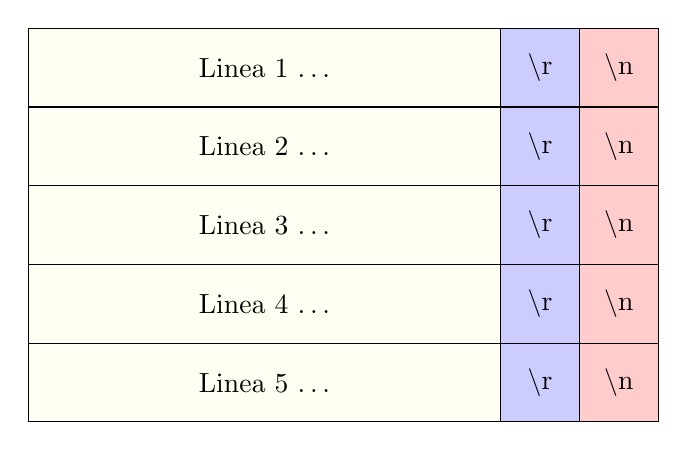
\begin{tikzpicture}
    \foreach \y in {1,...,5} {
    \filldraw[fill=yellow!05!white] (0,5-\y) rectangle node {Linea \y\  $\dots$} (6,5-\y+1);
    \filldraw[fill=blue!20!white] (6,5-\y) rectangle node {\textbackslash r} (7,5-\y+1);
    \filldraw[fill=red!20!white] (7,5-\y) rectangle node {\textbackslash n} (8,5-\y+1);
}
\end{tikzpicture}
\caption{Conteo de lineas}
\end{figure}

\subsection*{Pedir por pantalla los datos que se van a ingresar}
Lo primero que se le pide al usuario es donde quiere ingresar el nuevo registro,
se espera un numero en decimal, para esto el programa cuenta la cantidad de
caracteres que son números del 0 al 9 y los pasa a un ciclo que convierte la
cadena de caracteres en un entero mediante multiplicaciones consecutivas por
10 y la suma de cada numero de la cadena. Finalmente se piden el resto de
caracteres que son simplemente cadenas de caracteres que se guardan en sus
variables especificas.


\subsection*{ Creacion del nuevo elemento que se anexara al archivo}
    Una vez obtenidos los datos, hace falta juntarlos de forma eficiente y en el
    formato indicato, esto se logra mediante la funcion de la api de windows
    \comillas{\textbf{lstrcat}} esta toma como parametros 2 direcciones a strings
    la primera es a la cual se anexará la segunda, de esta forma solo hace falta
    llamarla tantas veces sea necesaria y con los parametros adecuados para
    construir nuestro nuevo registro.


\begin{figure}[!ht]
\centering
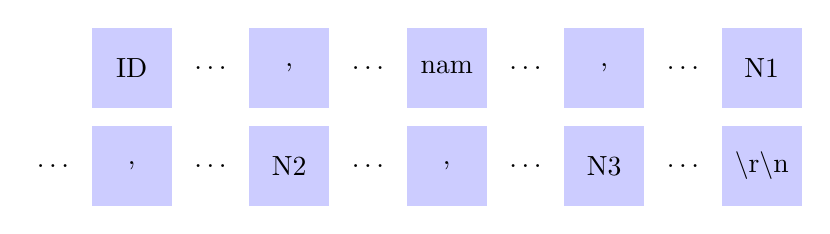
\begin{tikzpicture}
    \filldraw[blue!20!white] (0,0) rectangle (1,1);
    \node at (0.5, 0.5) {ID};
\foreach \x\y in {1/{,},2/nam,3/{,},4/N1}{
    \node at (2*\x - 0.5,0.5) {$\dots$};
    \filldraw[blue!20!white] (2*\x,0) rectangle (2*\x + 1,1);
    \node at (2*\x + 0.5, 0.5) {\y};
}

    \foreach \x\y in {0/{,},1/{N2},2/{,},3/N3, 4/{\textbackslash r\textbackslash n}}{
    \node at (2*\x - 0.5,-0.75) {$\dots$};
    \filldraw[blue!20!white] (2*\x,-1.25) rectangle (2*\x + 1,-0.25);
    \node at (2*\x + 0.5,-0.75) {\y};
}
\end{tikzpicture}
\caption{Creando registro}
\end{figure}


\subsection*{Localizacion de la posicion en la que se escribira}

    Para esto se utilizan los elementos guardados anteriormente, al hacer
    \comillas{pop} se retornan los valores numericos de donde se va a insertar
    el nuevo registro y cuantas lineas tiene el archivo. se hace una estructura
    de decision anidada en la cual se evaluan 3 posibilidades:

    \begin{itemize}
        \item El elemento se agregara en la primera posicion.
        \item El elemento se agregara en una posicion intermedia.
        \item El elemento se agregara en la ultima posicion.
    \end{itemize}

    Si se anexara al inicio o al final es una decision trivial, simplemente se
    estructura de esa forma la concatenacion y se envia al segmento de escritura
    correspondiente. En el caso de que el elemento sea
    en una posicion intermedia se utiliza un ciclo parecido al del conteo de lineas
    con la unica modificacion de que al conseguirse una nueva linea se evalua si
    es en esta linea en donde se anexara el registro creado anteriormente; si es
    asi, se va al procedimiento de escritura, si no se continua el ciclo hasta
    conseguir la linea deseada.

\begin{figure}[!ht]
\centering
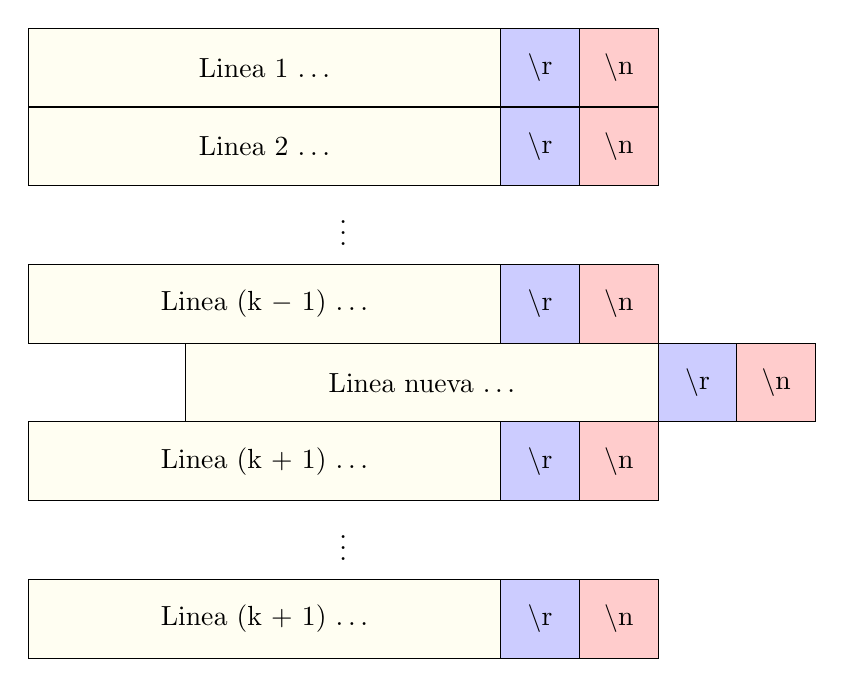
\begin{tikzpicture}

\filldraw[fill=yellow!05!white] (0,1) rectangle node {Linea 1 $\dots$} (6,2);
\filldraw[fill=blue!20!white] (6,1) rectangle node {\textbackslash r} (7,2);
\filldraw[fill=red!20!white] (7,1) rectangle node {\textbackslash n} (8,2);


\filldraw[fill=yellow!05!white] (0,0) rectangle node {Linea 2  $\dots$} (6,1);
\filldraw[fill=blue!20!white] (6,0) rectangle node {\textbackslash r} (7,1);
\filldraw[fill=red!20!white] (7,0) rectangle node {\textbackslash n} (8,1);


\node at (4,-0.5) {$\vdots$};

\filldraw[fill=yellow!05!white] (0,-2) rectangle node {Linea (k $-$ 1)  $\dots$} (6,-1);
\filldraw[fill=blue!20!white] (6,-2) rectangle node {\textbackslash r} (7,-1);
\filldraw[fill=red!20!white] (7,-2) rectangle node {\textbackslash n} (8,-1);

\filldraw[fill=yellow!05!white] (0,-2) rectangle node {Linea (k $-$ 1)  $\dots$} (6,-1);
\filldraw[fill=blue!20!white] (6,-2) rectangle node {\textbackslash r} (7,-1);
\filldraw[fill=red!20!white] (7,-2) rectangle node {\textbackslash n} (8,-1);

\filldraw[fill=yellow!05!white] (2,-3) rectangle node {Linea nueva  $\dots$} (8,-2);
\filldraw[fill=blue!20!white] (8,-3) rectangle node {\textbackslash r} (9,-2);
\filldraw[fill=red!20!white] (9,-3) rectangle node {\textbackslash n} (10,-2);

%\draw[very thick, blue,->] (1.75,-2.5) -- (0.5,-2.5);

\filldraw[fill=yellow!05!white] (0,-4) rectangle node {Linea (k + 1)  $\dots$} (6,-3);
\filldraw[fill=blue!20!white] (6,-4) rectangle node {\textbackslash r} (7,-3);
\filldraw[fill=red!20!white] (7,-4) rectangle node {\textbackslash n} (8,-3);

\node at (4,-4.5) {$\vdots$};

\filldraw[fill=yellow!05!white] (0,-6) rectangle node {Linea (k + 1)  $\dots$} (6,-5);
\filldraw[fill=blue!20!white] (6,-6) rectangle node {\textbackslash r} (7,-5);
\filldraw[fill=red!20!white] (7,-6) rectangle node {\textbackslash n} (8,-5);

\end{tikzpicture}
\caption{Colocando nuevo elemento en una posicion intermedia}
\end{figure}



\subsection*{ Escritura y cierre del fichero}

    Siguiendo las ideas anteriores, se presentan 3 posibilidades de escritura:

    \begin{itemize}
        \item Primera linea:
                se escribe 3 veces en el archivo:
                \begin{itemize}
                    \item Se escribe el nuevo registro.
                    \item Se escribe el salto de linea.
                    \item Se escribe el archivo leido.
                \end{itemize}
        \item Linea intermedia:
            Ocurre en cuatro pasos:
            \begin{itemize}
                    \item Se cuenta la cantidad de bytes a escribir de
                        acuerdo a la linea que se desea ingresar.
                    \item Se escribe esa cantidad bytes del archivo anterior.
                    \item Se escribe el nuevo registro.
                    \item Se escribe el resto del archivo.
            \end{itemize}

        \item Ultima linea:
            se escribe 3 veces en el archivo:
            \begin{itemize}
                \item Se escribe el archivo leido.
                \item Se escribe el salto de linea.
                \item Se escribe el nuevo registro.
            \end{itemize}
    \end{itemize}


\lstinputlisting[language={[x86masm]Assembler}]{practica5/consola/lectura.asm}

\section*{Funcionamiento del programa}

\begin{figure}[H]
  \includegraphics[width=\linewidth]{practica5/img/fig1}
    \caption{Abriendo el archivo}
\end{figure}

\begin{figure}[H]
  \includegraphics[width=\linewidth]{practica5/img/fig2}
    \caption{Agregando un nuevo registro}
\end{figure}

\begin{figure}[H]
  \includegraphics[width=\linewidth]{practica5/img/fig3}
    \caption{Mostrando en pantalla el archivo resultante}
\end{figure}
